% =====================================================================
%  BÁO CÁO ĐỒ ÁN CUỐI KỲ — UIT (ĐHQG-HCM)
%  Bản LaTeX chuyển tự động từ Bao_Cao_Cuoi_Ky_UIT.docx
%  Biên dịch: XeLaTeX (xelatex -> bibtex -> xelatex -> xelatex)
%  Định dạng: A4, lề Trên/Dưới 2.0cm · Trái 3.0cm · Phải 2.0cm, TNR 13pt, dãn dòng 1.4
% =====================================================================
\documentclass[13pt,a4paper]{extreport}

\usepackage{fontspec}
\setmainfont{Times New Roman}
\usepackage[vietnamese]{babel}
\usepackage{amsmath,amssymb}

\usepackage[a4paper,top=2.0cm,bottom=2.0cm,left=3.0cm,right=2.0cm]{geometry}

\usepackage{setspace}
\setstretch{1.4}
\setlength{\parindent}{1.0cm}
\setlength{\parskip}{6pt}

\usepackage{graphicx}
\usepackage{float}
\usepackage{array}
\usepackage{tabularx}
\usepackage{longtable}
\usepackage[font=small,labelfont=bf,justification=centering]{caption}

\usepackage{indentfirst}
\usepackage{enumitem}
\setlist{nosep,leftmargin=1.2cm}

\usepackage{titlesec}
\titleformat{\chapter}[block]
  {\normalfont\bfseries\centering\fontsize{15}{18}\selectfont}
  {CHƯƠNG \thechapter.}{0.5em}{}
\titlespacing*{\chapter}{0pt}{0pt}{16pt}
\titleformat{\section}{\normalfont\bfseries\fontsize{13}{16}\selectfont}{\thesection.}{0.5em}{}
\titlespacing*{\section}{0pt}{12pt}{6pt}
\titleformat{\subsection}{\normalfont\bfseries\fontsize{13}{16}\selectfont}{\thesubsection.}{0.5em}{}
\titlespacing*{\subsection}{0pt}{10pt}{4pt}

\usepackage{fancyhdr}
\pagestyle{fancy}
\fancyhf{}
\cfoot{\thepage}
\renewcommand{\headrulewidth}{0pt}
\renewcommand{\footrulewidth}{0pt}

\usepackage[hidelinks,unicode]{hyperref}

\renewcommand{\contentsname}{MỤC LỤC}
\renewcommand{\listfigurename}{DANH SÁCH BIỂU ĐỒ}
\renewcommand{\listtablename}{DANH SÁCH BẢNG}
\renewcommand{\figurename}{Hình}
\renewcommand{\tablename}{Bảng}

\begin{document}

% ---------------------------------------------------------------------
%  TRANG BÌA
% ---------------------------------------------------------------------
\begin{titlepage}
\centering
{\bfseries\fontsize{13}{16}\selectfont ĐẠI HỌC QUỐC GIA THÀNH PHỐ HỒ CHÍ MINH\par}
\vspace{2pt}
{\bfseries\fontsize{14}{17}\selectfont TRƯỜNG ĐẠI HỌC CÔNG NGHỆ THÔNG TIN\par}
\vspace{6pt}
{\bfseries\fontsize{13}{16}\selectfont KHOA HỆ THỐNG THÔNG TIN\par}
\vspace{2.4cm}
{\bfseries\fontsize{15}{18}\selectfont BÁO CÁO ĐỒ ÁN CUỐI KỲ\par}
\vspace{0.3cm}
{\fontsize{13}{16}\selectfont Môn học: <TÊN MÔN HỌC> (mã lớp CS114)\par}
\vspace{1.0cm}
{\bfseries\fontsize{13}{16}\selectfont ĐỀ TÀI\par}
\vspace{0.4cm}
{\bfseries\fontsize{15}{18}\selectfont DỰ BÁO SUY GIẢM TÀI CHÍNH DOANH NGHIỆP\\[2pt]
BÁN LẺ TỪ DỮ LIỆU SEC XBRL BẰNG HỌC MÁY\par}
\vspace{1.4cm}
\begin{flushleft}
{\fontsize{13}{16}\selectfont Giảng viên hướng dẫn: <ThS. …………………>\par}
\vspace{0.4cm}
{\fontsize{13}{16}\selectfont Sinh viên thực hiện:\par}
\vspace{0.2cm}
{\fontsize{13}{16}\selectfont <Họ và tên> --- <MSSV>\par}
{\fontsize{13}{16}\selectfont <Họ và tên> --- <MSSV>\par}
{\fontsize{13}{16}\selectfont <Họ và tên> --- <MSSV>\par}
{\fontsize{13}{16}\selectfont <Họ và tên> --- <MSSV>\par}
\end{flushleft}
\vfill
{\bfseries\fontsize{13}{16}\selectfont TP. Hồ Chí Minh, tháng <…> năm <…>\par}
\end{titlepage}
\clearpage


\chapter*{LỜI CẢM ƠN}

\addcontentsline{toc}{chapter}{Lời cảm ơn}

Nhóm chúng em xin chân thành cảm ơn giảng viên hướng dẫn đã định hướng đề tài, góp ý về cách kiểm chứng dữ liệu và cách báo cáo kết quả trung thực — đặc biệt là yêu cầu kiểm tra dữ liệu về tận nguồn thay vì tin vào kết quả in ra. Chúng em cũng cảm ơn quý thầy cô Khoa Hệ thống Thông tin đã trang bị nền tảng về khai phá dữ liệu, học máy và đánh giá mô hình để nhóm hoàn thành đồ án. Cảm ơn các bạn trong lớp đã phản biện, chỉ ra những điểm số chưa hợp lý trong các bản báo cáo trước. Báo cáo còn nhiều hạn chế, nhóm mong nhận được góp ý.

\clearpage

\tableofcontents

\clearpage

\chapter*{DANH MỤC CHỮ VIẾT TẮT}

\addcontentsline{toc}{chapter}{Danh mục chữ viết tắt}

\begin{table}[H]
\centering
\begin{center}
\small
\begin{tabular}{|l|c|}
\hline
\textbf{Từ viết tắt} & \textbf{Diễn giải} \\ \hline
10-K / 10-Q & Báo cáo thường niên / báo cáo quý nộp cho SEC \\ \hline
8-K & Báo cáo sự kiện bất thường nộp cho SEC \\ \hline
AP & Average Precision (diện tích dưới đường Precision–Recall, PR-AUC) \\ \hline
AUROC & Diện tích dưới đường cong ROC \\ \hline
CI & Khoảng tin cậy (Confidence Interval) \\ \hline
CV & Kiểm định chéo (Cross-Validation) \\ \hline
EDA & Phân tích khám phá dữ liệu (Exploratory Data Analysis) \\ \hline
FN / FP & Bỏ sót (False Negative) / Báo động giả (False Positive) \\ \hline
GroupKFold / LOCO & Chia fold theo nhóm thực thể / giữ trọn một công ty ra ngoài \\ \hline
HGB & HistGradientBoostingClassifier (scikit-learn) \\ \hline
IR & Imbalance Ratio (tỉ lệ lớp đa số chia lớp thiểu số) \\ \hline
MCC & Matthews Correlation Coefficient \\ \hline
MD\&A & Management Discussion \& Analysis (thuyết minh trong 10-K/10-Q) \\ \hline
MLP & Mạng nơ-ron nhiều lớp (Multi-Layer Perceptron) \\ \hline
OOF & Out-of-fold (dự đoán ngoài fold khi kiểm định chéo) \\ \hline
RF & Random Forest \\ \hline
SEC & U.S. Securities and Exchange Commission \\ \hline
SHAP & SHapley Additive exPlanations (diễn giải mô hình) \\ \hline
VIF & Variance Inflation Factor (đo đa cộng tuyến) \\ \hline
XBRL & eXtensible Business Reporting Language (chuẩn gắn thẻ báo cáo tài chính) \\ \hline
\end{tabular}
\end{center}
\end{table}

\clearpage

\phantomsection\addcontentsline{toc}{chapter}{Danh sách bảng}

\listoftables

\clearpage

\phantomsection\addcontentsline{toc}{chapter}{Danh sách biểu đồ}

\listoffigures

\clearpage

\chapter{MỞ ĐẦU}

\section{Lý do chọn đề tài}

Ngành bán lẻ có cấu trúc tài chính đặc thù: biên lợi nhuận ròng mỏng, vốn lưu động quay nhanh, hàng tồn kho chiếm tỉ trọng lớn và chi phí thuê mặt bằng cố định. Ba đặc điểm này khiến một cú sốc doanh thu tương đối nhỏ cũng có thể đẩy doanh nghiệp vào trạng thái căng thẳng. Trong bộ dữ liệu của đồ án, điều này quan sát được trực tiếp: \texttt{debt\_to\_assets} có trung vị 0,72 — hơn một nửa số quý khảo sát có nợ phải trả chiếm trên 70\% tổng tài sản; \texttt{inventory\_to\_sales} trung vị 0,64. Khi doanh thu đi ngang hoặc giảm, đòn bẩy cao khuếch đại rủi ro rất nhanh.

Bài toán vì vậy là: từ báo cáo tài chính đã công bố, dự báo trước một quý liệu doanh nghiệp có rơi vào suy giảm tài chính hay không. Đây không phải câu hỏi mới (Beaver 1966, Altman 1968), nhưng dữ liệu XBRL của SEC nay miễn phí và có cấu trúc nên có thể làm lại ở quy mô tự động.

\section{Tính cấp thiết của vấn đề}

Hệ quả của việc phát hiện muộn là không đối xứng. Với một chuỗi bán lẻ, chậm một-hai quý có thể đồng nghĩa mất khả năng đàm phán với nhà cung cấp hoặc phải huy động vốn ở điều kiện bất lợi. Với phía cho vay/đầu tư, bỏ sót một ca suy giảm (FN) đắt hơn nhiều lần so với một báo động giả (FP); đồ án định lượng giả định \texttt{COST\_FN = 5}, \texttt{COST\_FP = 1} và dùng chính giả định này để chọn ngưỡng quyết định ở mục 3.4.3 thay vì lấy 0,5 theo thói quen.

Cách làm thủ công — đọc từng 10-K/10-Q và tự tách chỉ tiêu — không mở rộng được. Điểm mấu chốt kỹ thuật là SEC XBRL gắn thẻ taxonomy cho từng dòng số liệu, nên có thể bóc tách theo \texttt{tag}, theo kỳ (\texttt{start}/\texttt{end}) và theo ngày công bố (\texttt{filed}) một cách xác định. Tự động hóa biến bài toán đọc hiểu thành bài toán dữ liệu.

\section{Mục tiêu nghiên cứu}

\begin{enumerate}
\item Pipeline dữ liệu tái lập được: tải \texttt{companyfacts} từ SEC, chuẩn hóa về chuỗi 16 chỉ tiêu theo quý, gán nhãn và chia tập có dải purge; mọi bước kiểm chứng được bằng SHA-256 và đối chiếu ngược về SEC.
\item Bộ đặc trưng tài chính có ý nghĩa kinh tế (thanh khoản, đòn bẩy, sinh lời, hiệu quả hoạt động, tăng trưởng và đặc trưng đường đi theo cửa sổ quý).
\item Huấn luyện, so sánh các họ mô hình phân loại và chọn cấu hình tốt nhất theo giao thức đánh giá chống thổi phồng (cross-company), báo cáo trung thực cả những chỗ mô hình KHÔNG hơn baseline.
\end{enumerate}

\section{Phạm vi và phương pháp nghiên cứu}

Phạm vi dữ liệu: 8 chuỗi bán lẻ niêm yết tại Mỹ (WMT, HD, LOW, ROST, DG, ORLY, DKS, FIVE), 332 quý tài chính, tạo thành 324 mẫu dự báo cho giai đoạn FY2015–FY2026. Đơn vị tiền được quy đổi minh họa 25.000 VND/USD chỉ để thống nhất đơn vị trình bày, không phải số liệu Việt Nam và không phải tỷ giá lịch sử.

Phương pháp: quy trình khai phá dữ liệu theo trình tự dữ liệu → đặc trưng → mô hình → đánh giá. Điểm kiểm soát quan trọng nhất nằm ở khâu đánh giá, vì nhãn hóa ra gần như là thuộc tính của từng công ty (mục 3.1.3): nhóm áp dụng chia tập theo thời gian, kiểm định chéo theo nhóm công ty (\texttt{GroupKFold}, \texttt{Leave-One-Company-Out}) và luôn đặt cạnh baseline không dùng mô hình.

\clearpage

\chapter{CƠ SỞ LÝ THUYẾT}

\section{Khái niệm kiệt quệ tài chính (financial distress)}

Trong tài chính doanh nghiệp, kiệt quệ tài chính là trạng thái doanh nghiệp không còn đủ khả năng tạo dòng tiền để thực hiện các nghĩa vụ nợ, hoặc đang phải chịu các dấu hiệu dẫn tới điều đó (lỗ ròng kéo dài, dòng tiền hoạt động âm, vốn lưu động âm, vốn chủ sở hữu âm). Thuật ngữ này rộng hơn "phá sản": một doanh nghiệp có thể ở trạng thái kiệt quệ tài chính trong nhiều quý mà vẫn chưa nộp đơn phá sản. Phân biệt này quan trọng với đồ án vì bộ dữ liệu thu thập được không chứa sự kiện phá sản nào (xem mục 3.1.3), nên bài toán được định vị là dự báo suy giảm tài chính, không phải dự báo phá sản.

\section{Dữ liệu SEC và định dạng XBRL}

Từ năm 2009, SEC yêu cầu các công ty đại chúng nộp báo cáo tài chính kèm theo phần XBRL — mỗi dòng số liệu được gắn một thẻ (tag) trong taxonomy US-GAAP. Kết quả là mỗi công ty có một file \texttt{companyfacts} (JSON) liệt kê toàn bộ fact theo taxonomy, tag và đơn vị. Mỗi fact mang cấu trúc (tag, kỳ bắt đầu \texttt{start}, kỳ kết thúc \texttt{end}, giá trị \texttt{val}, số hiệu hồ sơ \texttt{accn}, ngày nộp \texttt{filed}).

Hai loại chỉ tiêu cần phân biệt khi bóc tách. Chỉ tiêu dạng số dư (instant) như \texttt{Assets}, \texttt{Liabilities}, \texttt{StockholdersEquity} chỉ có \texttt{end} và đặc trưng cho một thời điểm. Chỉ tiêu dạng số phát sinh (duration) như \texttt{Revenues}, \texttt{NetIncomeLoss}, \texttt{NetCashProvidedByOperatingActivities} có cả \texttt{start} và \texttt{end}. Nếu lấy nhầm fact luỹ kế từ đầu năm (year-to-date) thay vì đúng một quý, con số sẽ bị phóng đại. Vì vậy pipeline của đồ án lọc theo đúng cửa sổ quý (70–105 ngày) và với các chỉ tiêu luỹ kế thì trừ fact luỹ kế hiện tại cho fact luỹ kế trước đó để ra giá trị của riêng quý.

\section{Từ Altman Z-score đến học máy}

Mô hình cổ điển của Altman (1968) gộp vài tỷ số kế toán thành một điểm số theo trọng số cố định. Với doanh nghiệp phi sản xuất, dịch vụ, biến thể Z''-score tính \texttt{Z = 6,56·(vốn lưu động/tổng tài sản) + 3,26·(lợi nhuận giữ lại/tổng tài sản) + 6,72·(EBIT/tổng tài sản) + 1,05·(giá trị sổ sách vốn chủ sở hữu/tổng nợ)}. Ưu điểm của nó là diễn giải được và không cần huấn luyện; hạn chế là trọng số được chọn từ một tập mẫu cũ, giả định quan hệ tuyến tính giữa các tỷ số và một ngưỡng chung cho mọi ngành.

Học máy thay thế hai giả định đó bằng cách học trọng số và mặt quyết định từ chính dữ liệu. Với 47 đặc trưng và tương tác phi tuyến (ví dụ: lợi nhuận giảm mạnh chỉ nguy hiểm khi đi kèm đòn bẩy cao), mô hình cây và mạng nơ-ron có cơ hội bắt được quan hệ mà một công thức tuyến tính bỏ lỡ. Đồ án vì vậy dùng Altman Z'' làm một baseline để so sánh (mục 3.4), thay vì thay thế nó bằng niềm tin.

\section{Thước đo đánh giá cho dữ liệu mất cân bằng}

Vấn đề đầu tiên là accuracy gây hiểu nhầm. Trên test của đồ án, lớp suy giảm chiếm 59,4\%; chỉ cần đoán tất cả là "suy giảm" đã đạt accuracy 59,4\% mà không phân biệt được gì. Vì vậy nhóm không dùng accuracy làm chỉ số chính, mà báo cáo:

\begin{enumerate}
\item \textbf{AUROC} — khả năng xếp hạng của điểm số, độc lập ngưỡng;
\item \textbf{AP (PR-AUC)} — diện tích dưới đường Precision–Recall, chỉ số phù hợp khi lớp thiểu số là lớp cần quan tâm;
\item \textbf{Precision / Recall / F1 và macro-F1} tại một ngưỡng cụ thể, cộng \textbf{MCC} để có một chỉ số duy nhất không bị lệch theo tỉ lệ lớp;
\item \textbf{Brier score} cho chất lượng hiệu chuẩn xác suất — cần thiết vì ngưỡng quyết định phụ thuộc xác suất, không chỉ thứ hạng.
\end{enumerate}

Vấn đề thứ hai là ngưỡng quyết định. Thay vì cố định 0,5, đồ án chọn ngưỡng tối thiểu hoá chi phí kỳ vọng \texttt{COST\_FN·FN + COST\_FP·FP} (lý thuyết quyết định). Về mặt đại số, nếu coi xác suất là hiệu chuẩn đúng, chi phí kỳ vọng tối thiểu tại \texttt{p* = COST\_FP/(COST\_FN + COST\_FP)}. Bước này được hiện thực trong \texttt{forecasting/evaluation.py::cost\_optimal\_threshold} và chỉ tính trên validation, không dùng test.

\clearpage

\chapter{HIỆN THỰC HỆ THỐNG VÀ KẾT QUẢ}

Chương này mô tả hệ thống đã hiện thực và kết quả đo được. Mọi con số trong chương đều lấy trực tiếp từ artifact sinh bởi mã nguồn (\texttt{reports/results/*.json}), có thể tái lập bằng \texttt{python -m scripts.run\_all}.

\section{Pipeline dữ liệu SEC XBRL và gán nhãn}

\subsection{Corpus và bóc tách companyfacts}

Nguồn dữ liệu là endpoint công khai \texttt{data.sec.gov/api/xbrl/companyfacts/CIK…json} do \texttt{scripts/crawl\_sec.py} tải về (kèm delay 0,15 giây để tôn trọng giới hạn tần suất của SEC). Mỗi công ty được lưu thành một file raw 5–8 MB và ghi lại SHA-256 trong \texttt{data/sec/downloads.json} để về sau đối chiếu được là file không bị sửa tay.

Từ 20 công ty ban đầu, nhóm giữ 8 công ty thoả hai điều kiện: có tối thiểu 32 quý (8 năm) báo cáo và đủ 16 chỉ tiêu chuẩn. Các công ty bị loại kèm lý do cụ thể nằm trong \texttt{data/retail-expanded/corpus.json} (ví dụ: đổi kỳ tài chính giữa chừng, hoặc thiếu quá 30\% số ô chỉ tiêu).

\begin{table}[H]
\centering
\caption{Corpus 8 doanh nghiệp bán lẻ và số quý dữ liệu}
\begin{center}
\footnotesize
\begin{tabular}{|l|c|c|c|c|}
\hline
\textbf{Ticker} & \textbf{Công ty} & \textbf{Số quý} & \textbf{Năm tài chính} & \textbf{Tỉ lệ nhãn = 1} \\ \hline
WMT & Walmart & 48 & FY2015–FY2026 & 100\% \\ \hline
HD & The Home Depot & 44 & FY2015–FY2026 & 100\% \\ \hline
LOW & Lowe's & 44 & FY2015–FY2026 & 100\% \\ \hline
ROST & Ross Stores & 44 & FY2015–FY2026 & 5\% \\ \hline
DG & Dollar General & 32 & FY2018–FY2026 & 55\% \\ \hline
ORLY & O'Reilly Automotive & 44 & FY2015–FY2026 & 91\% \\ \hline
DKS & Dick's Sporting Goods & 44 & FY2015–FY2026 & 12\% \\ \hline
FIVE & Five Below & 32 & FY2018–FY2026 & 19\% \\ \hline
\end{tabular}
\end{center}
\end{table}

Tổng cộng 16 chỉ tiêu × 332 quý = 5.312 ô dữ liệu. Bước kiểm chứng (\texttt{scripts/verify\_provenance.py}) mở lại từng file raw và tra ngược từng ô: 4.609 ô có fact tương ứng trong companyfacts (kèm \texttt{accn}, \texttt{form}, ngày \texttt{filed}), 703 ô không có fact ở SEC nên được để \texttt{null}. Số fact thiếu trong SEC: 0; số ô bịa số (không có fact mà vẫn có giá trị): 0; số hash lệch registry: 0. Nói cách khác, mọi con số dùng để huấn luyện đều truy được về nguồn công khai.

\subsection{Chuẩn hóa kỳ kế toán}

Với chỉ tiêu số dư (instant), giá trị là con số tại ngày \texttt{end}. Với chỉ tiêu số phát sinh (duration), pipeline chỉ nhận fact có độ dài kỳ trong khoảng 70–105 ngày — tương ứng một quý 13 tuần — nhằm loại các fact luỹ kế. Trường hợp chỉ tiêu chỉ được công bố dạng luỹ kế từ đầu năm, mã trong \texttt{scripts/prepare\_sec.py} trừ luỹ kế hiện tại cho luỹ kế của kỳ liền trước (\texttt{current\_ytd\_minus\_previous\_ytd}) để ra giá trị quý riêng, đồng thời kiểm tra hai fact luỹ kế phải cùng mốc bắt đầu năm.

Một điểm phải xử lý riêng là thẻ \texttt{liabilities}: chỉ 39\% số quý có tag này (có công ty dưới 16\%). Nếu bỏ qua, hai đặc trưng \texttt{debt\_to\_assets} và \texttt{debt\_to\_equity} sẽ là NaN ở phần lớn mẫu và mô hình mất hẳn thông tin đòn bẩy. Vì vậy nhóm suy nợ phải trả từ đẳng thức kế toán \texttt{nợ = tổng tài sản − vốn chủ sở hữu} khi thiếu tag, và đối chiếu lại 124 quý có tag: 122 khớp tuyệt đối, 2 quý lệch do nộp lại báo cáo (restatement).

\subsection{Định nghĩa nhãn}

Nhãn gốc \texttt{is\_distressed} là trạng thái của quý target (quý mà mô hình phải dự báo). Điều đáng chú ý là nhãn này KHÔNG tái tạo được từ 16 chỉ tiêu công bố: thử 9 quy tắc kế toán đơn giản, quy tắc khớp cao nhất (\texttt{stress\_signals} ≥ 1 tín hiệu) chỉ đạt 74,7\%, các quy tắc đơn chỉ tiêu chỉ 39–65\%. Nhóm chấp nhận điều này như một hạn chế của bộ dữ liệu và xử lý bằng hai cách: (i) kiểm chứng độ nhạy với các định nghĩa nhãn tái lập được (mục 3.4.5); (ii) ghi rõ giới hạn trong báo cáo thay vì che đi.

Nhóm cũng kiểm tra khả năng có sự kiện phá sản thật bằng cách đọc hồ sơ 8-K (\texttt{scripts/fetch\_events.py}): trong 8/8 công ty, số sự kiện phá sản (8-K item 1.03) là 0. Vì vậy bài toán được định vị chính danh là dự báo suy giảm tài chính, không phải dự báo phá sản.

\subsection{Chia tập dữ liệu và dải purge}

Mỗi mẫu là một cặp (lịch sử các quý đã công bố trước \texttt{as\_of}, quý target cần dự báo, nhãn). Việc chia tập theo thời gian trong từng công ty: 8 quý cuối là test, 4 quý liền trước là validation, phần còn lại là train. Giữa các tập có dải purge: mỗi công ty bỏ ra 1 quý ngay trước validation và 1 quý ngay sau validation để tránh rò rỉ nhãn do cửa sổ lịch sử chồng lấn. Kết quả: train 212 mẫu, validation 32, test 64, purged 16; tất cả dùng chung một chính sách nên so sánh được giữa các mô hình.

\clearpage

\section{Kỹ thuật trích xuất đặc trưng (feature engineering)}

Bộ đặc trưng gồm 47 cột, hiện thực thuần numpy trong \texttt{forecasting/features.py} (\texttt{build\_feature\_matrix}, \texttt{feature\_names}). Nguyên tắc xuyên suốt là không rò rỉ: chỉ dùng các quý đã công bố trước \texttt{as\_of}, mọi tỷ số và tăng trưởng tính trong cửa sổ lịch sử tối đa 8 quý, không nhìn vào quý target hay nhãn.

\subsection{Đặc điểm dữ liệu quan sát trước khi tạo đặc trưng}

Hai đặc điểm dữ liệu định hình toàn bộ thiết kế phía sau. Thứ nhất, mất cân bằng lớp ở cấp mẫu chỉ ở mức nhẹ (lớp suy giảm chiếm 62,3\% train, IR = 1,65), nhưng ở cấp công ty thì rất nặng: HD, LOW, WMT có 100\% quý mang nhãn 1; ROST chỉ 4,7\%. Điều này có nghĩa nhãn gần như là thuộc tính của từng công ty — nên mọi đánh giá phải chia theo nhóm công ty. Thứ hai, phân phối các tỷ số lệch mạnh: trong 14 tỷ số, 6 tỷ số có |skew| > 1, nặng nhất là \texttt{debt\_to\_equity} (skew −14,9) với 30,6\% giá trị nằm ngoài khoảng IQR.

\begin{figure}[H]
\centering
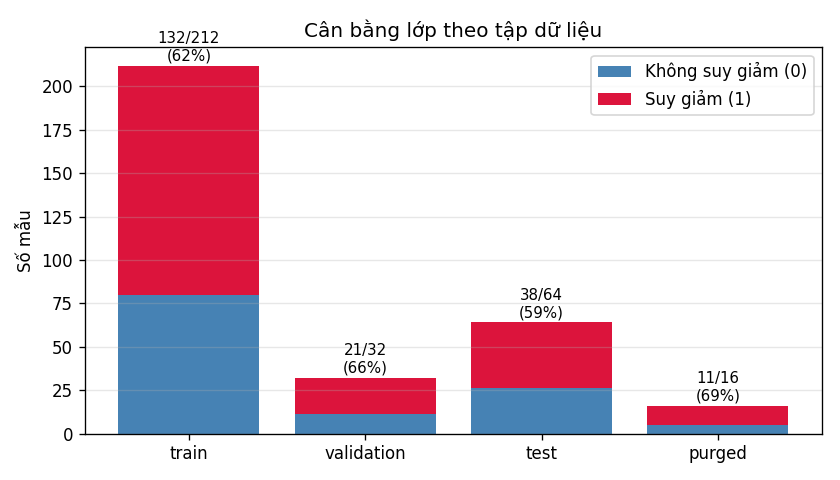
\includegraphics[width=0.8\textwidth]{figures/02_class_balance.png}
\caption{Cân bằng lớp theo tập dữ liệu}
\end{figure}

\begin{figure}[H]
\centering
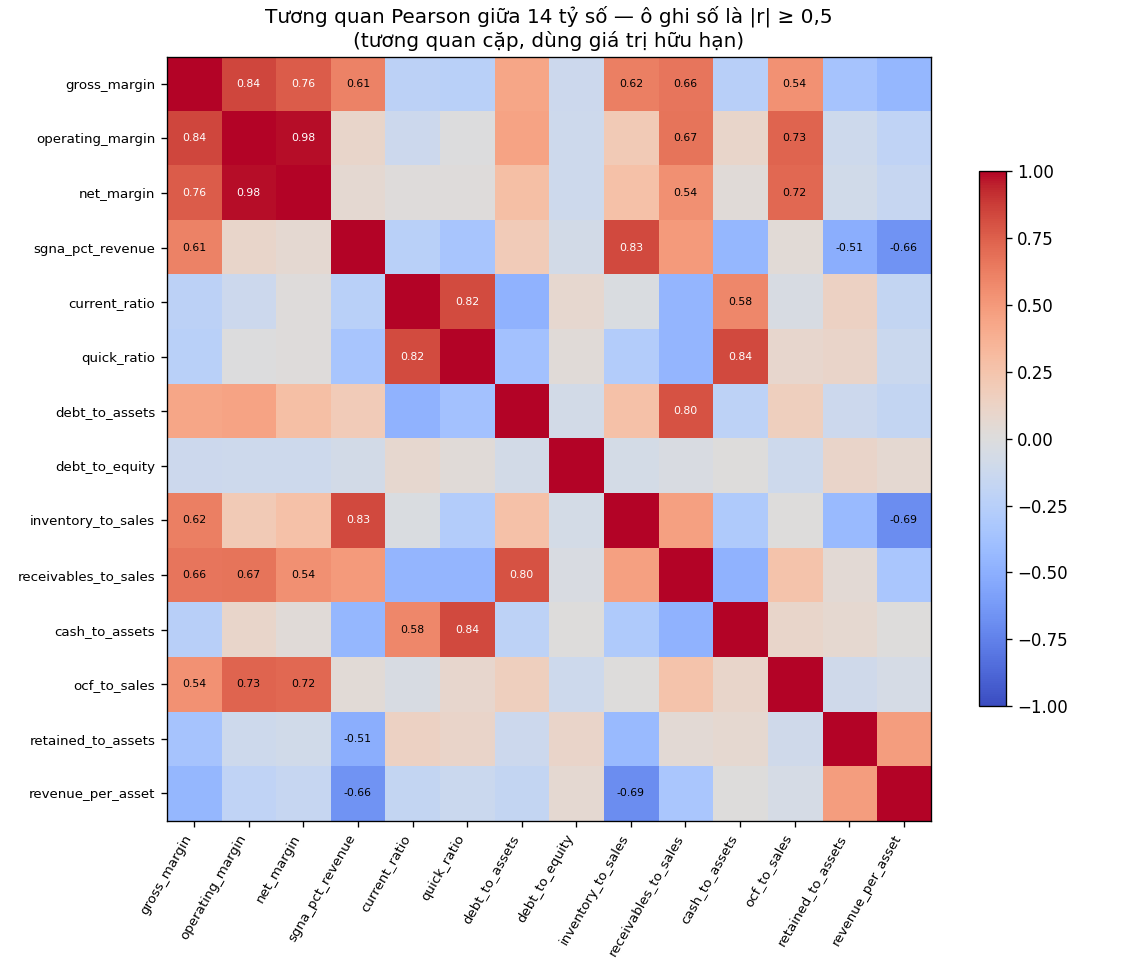
\includegraphics[width=0.8\textwidth]{figures/08_ratio_correlation.png}
\caption{Tương quan giữa các tỷ số tài chính}
\end{figure}

\subsection{Mười bốn tỷ số tài chính}

Các tỷ số (từ điển \texttt{RATIOS} trong \texttt{forecasting/config.py}) chia bốn nhóm kinh tế:

\begin{itemize}
\item \textbf{Thanh khoản:} \texttt{current\_ratio} = tài sản ngắn hạn / nợ ngắn hạn; \texttt{quick\_ratio} = (tài sản ngắn hạn − hàng tồn kho) / nợ ngắn hạn.
\item \textbf{Đòn bẩy:} \texttt{debt\_to\_assets} = nợ / tổng tài sản; \texttt{debt\_to\_equity} = nợ / vốn chủ sở hữu.
\item \textbf{Sinh lời:} \texttt{gross\_margin} = (doanh thu − giá vốn) / doanh thu; \texttt{operating\_margin} = lợi nhuận hoạt động / doanh thu; \texttt{net\_margin} = lợi nhuận ròng / doanh thu; \texttt{retained\_to\_assets} = lợi nhuận giữ lại / tổng tài sản.
\item \textbf{Hiệu quả hoạt động:} \texttt{inventory\_to\_sales}, \texttt{receivables\_to\_sales}, \texttt{revenue\_per\_asset}, \texttt{ocf\_to\_sales} (dòng tiền hoạt động / doanh thu), \texttt{sgna\_pct\_revenue}, \texttt{cash\_to\_assets}.
\end{itemize}

Mỗi tỷ số được đưa vào mô hình ở hai dạng: giá trị của quý gần nhất (\texttt{*\_latest}) và mức thay đổi so với cùng kỳ năm trước (\texttt{*\_yoy}), tức 14 × 2 = 28 cột.

\subsection{Tăng trưởng, cấu trúc vốn và đặc trưng đường đi}

Nhóm tăng trưởng gồm 10 cột \texttt{*\_yoy\_growth} cho các chỉ tiêu chính. Nhóm cấu trúc vốn có \texttt{working\_capital\_to\_assets}. Nhóm đường đi (nhóm \texttt{path}) là phần được thiết kế riêng cho bài toán này: vì suy giảm tài chính là một quá trình chứ không phải trạng thái của một quý, nhóm đưa vào các cực trị xấu nhất trong cửa sổ và số quý âm liên tiếp — \texttt{current\_ratio\_min\_window}, \texttt{ocf\_to\_sales\_min\_window}, \texttt{net\_margin\_min\_window}, \texttt{revenue\_drawdown\_window} (mức tụt so với đỉnh doanh thu), \texttt{negative\_ni\_streak}, \texttt{negative\_ocf\_streak}.

\begin{table}[H]
\centering
\caption{Cấu trúc 47 đặc trưng theo nhóm}
\begin{center}
\small
\begin{tabular}{|l|c|c|}
\hline
\textbf{Nhóm} & \textbf{Số cột} & \textbf{Nội dung} \\ \hline
ratios\_latest & 14 & 14 tỷ số tại quý gần nhất \\ \hline
ratios\_yoy & 14 & Mức thay đổi 14 tỷ số so với cùng kỳ năm trước \\ \hline
growth & 10 & Tăng trưởng YoY của 10 chỉ tiêu chính \\ \hline
structure & 1 & working\_capital\_to\_assets \\ \hline
stress & 2 & distress\_quarters\_in\_window, revenue\_cv \\ \hline
path & 6 & Cực trị xấu nhất trong cửa sổ + số quý âm liên tiếp \\ \hline
\textbf{Tổng} & \textbf{47} &  \\ \hline
\end{tabular}
\end{center}
\end{table}

\subsection{Xử lý giá trị khuyết và ngoại lai}

Giá trị khuyết được giữ nguyên dưới dạng NaN qua tầng đặc trưng, rồi xử lý bên trong pipeline bằng \texttt{SimpleImputer(strategy='median')} — median được tính chỉ trên train. Với ngoại lai, đồ án thử \texttt{Winsorizer} (clip theo IQR hoặc P1–P99, ngưỡng học từ train) như một biến thể và báo cáo kết quả âm: trên đúng mô hình được chốt (Random Forest), winsorize = IQR cải thiện cross-company AP chỉ +0,13 điểm \% (0,9590 so với 0,9577) — nằm trong khoảng nhiễu của 244 mẫu out-of-fold. Vì vậy pipeline chính giữ không winsorize cho đơn giản và dễ diễn giải; winsorize chỉ dùng như một ablation. Kết quả tương tự với lựa chọn scaler: \texttt{StandardScaler} và \texttt{RobustScaler} chênh nhau dưới 0,5 điểm \% AP cross-company.

\clearpage

\section{Thiết kế mô hình}

\subsection{Bốn họ mô hình}

Đồ án cố tình chọn bốn họ mô hình khác nhau về cơ chế học để trả lời câu hỏi "bài toán cần loại giả thuyết nào", thay vì thử nhiều biến thể của cùng một họ: tuyến tính (Logistic Regression), bagging cây (Random Forest), boosting cây (HistGradientBoosting) và mạng nơ-ron phi tuyến không dựa trên cây (MLP). Toàn bộ dùng thư viện \texttt{scikit-learn}; đồ án không dùng \texttt{xgboost}/\texttt{lightgbm} trong pipeline chính.

\begin{table}[H]
\centering
\caption{Siêu tham số 4 họ mô hình}
\begin{center}
\small
\begin{tabular}{|l|c|c|}
\hline
\textbf{Mô hình} & \textbf{Lớp scikit-learn} & \textbf{Siêu tham số mặc định} \\ \hline
Logistic Regression & LogisticRegression & max\_iter=2000, C=0,1 \\ \hline
Random Forest & RandomForestClassifier & n\_estimators=300, max\_depth=6, min\_samples\_leaf=2, class\_weight=balanced\_subsample \\ \hline
HistGradientBoosting & HistGradientBoostingClassifier & max\_iter=300, learning\_rate=0,05, max\_depth=3, l2\_regularization=1,0, class\_weight=balanced \\ \hline
MLP & MLPClassifier & hidden\_layer\_sizes=32, alpha=1e-3, learning\_rate\_init=1e-3, early\_stopping=True \\ \hline
\end{tabular}
\end{center}
\end{table}

Lưu ý kỹ thuật với mất cân bằng: \texttt{RandomForestClassifier} và \texttt{HistGradientBoostingClassifier} nhận \texttt{class\_weight} nên trọng số lớp được truyền trực tiếp. \texttt{MLPClassifier} không có \texttt{class\_weight}, nên mất cân bằng được xử lý bằng ngưỡng/cost-sensitive ở tầng đánh giá thay vì nhồi trọng số giả vào mô hình.

\subsection{Pipeline và chống rò rỉ}

Mỗi mô hình là một \texttt{sklearn.pipeline.Pipeline}: \texttt{[winsorize] → SimpleImputer(median) → [scaler] → model} (\texttt{forecasting/models.py::make\_model}). Đặt impute/scale bên trong Pipeline có tác dụng chặn rò rỉ: thống kê impute/scale chỉ được \texttt{fit} trên train, khi kiểm định chéo chỉ trên fold-train. Scaler mặc định là \texttt{StandardScaler} cho mô hình tuyến tính/MLP và \texttt{none} cho mô hình cây; có thể đổi sang \texttt{RobustScaler}/\texttt{PowerTransformer}/\texttt{QuantileTransformer} qua tham số \texttt{scaler}. Biến môi trường \texttt{RANDOM\_SEED = 42} cố định để tái lập.

\subsection{Quy tắc chọn mô hình}

Nếu chọn mô hình theo AUROC in-domain, kết quả sẽ bị chi phối bởi "nhớ mặt công ty" — baseline ticker-prior đạt AUROC 0,986 (mục 3.4.2). Vì vậy nhóm chọn theo thứ tự ưu tiên: \textbf{AP cross-company} (GroupKFold trên train+validation) → best-F1(validation) → AP(validation) → AUROC(validation) → gap overfit nhỏ nhất. Quy tắc này được mã hóa tại \texttt{forecasting/train.py::\_rank} và ghi lại trong \texttt{summary.json} để kiểm chứng được.

\subsection{Tinh chỉnh siêu tham số}

Tinh chỉnh dùng kiểm định chéo chia theo công ty (\texttt{GroupKFold}) và chọn theo AP, để không lặp lại sai lầm chọn theo metric in-domain. Nhận xét trung thực: kết quả tinh chỉnh chênh lệch rất nhỏ so với cấu hình mặc định — mô hình RF tốt nhất (\texttt{max\_depth=3, n\_estimators=500}) chỉ hơn mặc định +0,3 điểm \% CV-AP, MLP hơn +4,6 điểm \% nhưng vẫn tụt hậu về cross-company. Vì vậy mô hình triển khai giữ cấu hình mặc định (đơn giản, ít nguy cơ overfit theo lựa chọn), và bảng tinh chỉnh được giữ lại như bằng chứng là nhóm đã thử.

\begin{table}[H]
\centering
\caption{Tinh chỉnh siêu tham số, CV chia theo công ty}
\begin{center}
\small
\begin{tabular}{|l|c|c|c|}
\hline
\textbf{Mô hình} & \textbf{Cấu hình tốt nhất} & \textbf{CV-AP} & \textbf{CV-AUROC} \\ \hline
logistic & C=0,01, class\_weight=None & 0,960 & 0,917 \\ \hline
random\_forest & max\_depth=3, min\_samples\_leaf=2, n\_estimators=500 & 0,989 & 0,976 \\ \hline
hist\_gradient\_boosting & learning\_rate=0,03, max\_depth=2, max\_iter=200 & 0,939 & 0,934 \\ \hline
mlp & alpha=1e-4, hidden\_layer\_sizes=64 & 0,845 & 0,750 \\ \hline
\end{tabular}
\end{center}
\end{table}

\clearpage

\section{Kết quả thực nghiệm}

Mọi so sánh dưới đây dùng \textbf{cùng tập test 64 mẫu (38 dương, 59,4\%)}, và test \textbf{không} tham gia vào bất kỳ bước chọn mô hình hay chọn ngưỡng nào. Ngưỡng vận hành của đồ án là 0,788, chọn trước đó trên validation bằng tiêu chí tối thiểu chi phí kỳ vọng.

\subsection{So sánh bốn họ mô hình}

\begin{table}[H]
\centering
\caption{Bốn họ mô hình trên test tại ngưỡng vận hành 0,788}
\begin{center}
\footnotesize
\begin{tabular}{|l|c|c|c|c|c|c|}
\hline
\textbf{Mô hình} & \textbf{AUROC} & \textbf{AP} & \textbf{F1@0,5} & \textbf{F1@0,788} & \textbf{MCC@0,788} & \textbf{TN/FP/FN/TP} \\ \hline
Logistic Regression & 0,983 & 0,989 & 0,935 & 0,914 & 0,827 & 26/0/6/32 \\ \hline
Random Forest & 0,983 & 0,991 & 0,949 & 0,960 & 0,904 & 25/1/2/36 \\ \hline
HistGradientBoosting & 0,977 & 0,987 & 0,937 & 0,907 & 0,775 & 23/3/4/34 \\ \hline
MLP & 0,971 & 0,982 & 0,914 & 0,895 & 0,741 & 22/4/4/34 \\ \hline
\end{tabular}
\end{center}
\end{table}

Random Forest là mô hình được chốt. Tại ngưỡng 0,788, nó đạt precision = 0,973, recall = 0,947, F1 = 0,960, accuracy = 0,953, specificity = 0,962 và Brier = 0,058. Đáng chú ý là toàn bộ bốn họ mô hình đều cho F1@0,5 khá cao (0,91–0,95) nhưng chỉ 1–2 mô hình giữ được F1 cao khi ngưỡng bị dịch lên 0,788 — nghĩa là thứ hạng điểm số giữa các mô hình không khác nhiều, khác biệt nằm ở vùng xác suất quanh ngưỡng quyết định.

\begin{figure}[H]
\centering
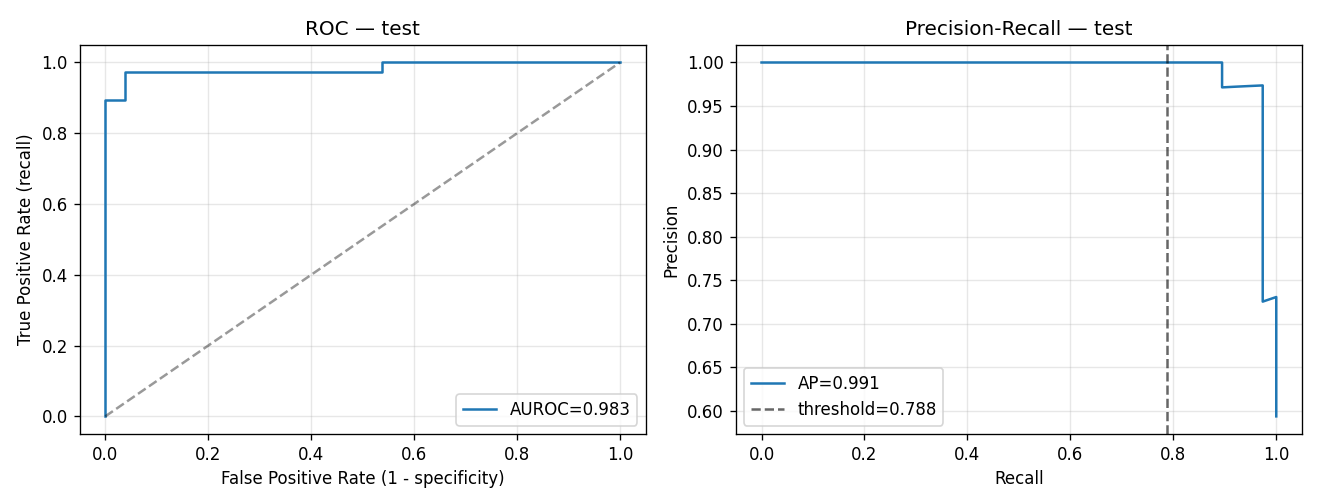
\includegraphics[width=0.8\textwidth]{figures/test_roc_pr_curves.png}
\caption{Đường ROC và Precision–Recall trên test}
\end{figure}

\subsection{So sánh với baseline và giao thức chống thổi phồng}

Phần này là điểm quan trọng nhất về mặt phương pháp của đồ án. Nếu chỉ nhìn AUROC ≈ 0,98, ta dễ kết luận mô hình rất tốt. Nhưng đặt cạnh một baseline không dùng mô hình — lấy tỉ lệ nhãn 1 trung bình trong train theo từng công ty (\texttt{ticker\_prior}) — mô hình gần như không hơn:

\begin{table}[H]
\centering
\caption{So sánh với các hệ thống đối chứng (test)}
\begin{center}
\small
\begin{tabular}{|l|c|c|}
\hline
\textbf{Hệ thống} & \textbf{AUROC} & \textbf{AP} \\ \hline
model[random\_forest] & 0,983 & 0,991 \\ \hline
ticker\_prior (baseline không học) & 0,986 & 0,985 \\ \hline
single\_feature[debt\_to\_assets\_latest] & 0,889 & 0,938 \\ \hline
rule[altman\_z\_double\_prime < 1,1] & 0,758 & 0,865 \\ \hline
dummy\_most\_frequent & 0,500 & 0,594 \\ \hline
\end{tabular}
\end{center}
\end{table}

Kết quả cho thấy baseline ticker-prior ngang bằng hoặc nhích hơn mô hình về AUROC (0,986 so với 0,983) và chỉ kém hơn về AP (0,985 so với 0,991). Quy tắc Altman Z'' (lấy mốc < 1,1) đạt AUROC 0,758 — thấp hơn rõ rệt, nhưng dùng công thức công khai, không học tham số và không cần train. Đọc cùng nhau, các con số này nói rằng 'AUROC cao' chưa chứng minh năng lực dự báo suy giảm.

Để tách phần 'nhớ mặt công ty' khỏi năng lực tổng quát hoá, nhóm đánh giá lại theo \texttt{GroupKFold} — giữ trọn một công ty ra ngoài train trong mỗi fold. Khoảng cách giữa hai cách đo chính là phần thổi phồng:

\begin{table}[H]
\centering
\caption{In-domain so với cross-company (GroupKFold)}
\begin{center}
\footnotesize
\begin{tabular}{|l|c|c|c|c|}
\hline
\textbf{Mô hình} & \textbf{AUROC in-domain} & \textbf{AP in-domain} & \textbf{AUROC cross-company} & \textbf{AP cross-company} \\ \hline
Random Forest & 0,983 & 0,991 & 0,933 & 0,957 \\ \hline
Logistic Regression & 0,983 & 0,989 & 0,912 & 0,942 \\ \hline
HistGradientBoosting & 0,977 & 0,987 & 0,926 & 0,953 \\ \hline
MLP & 0,971 & 0,982 & 0,789 & 0,832 \\ \hline
\end{tabular}
\end{center}
\end{table}

Hai điểm cần nói thẳng. Thứ nhất, khi giữ công ty ra ngoài, AUROC của mô hình chốt giảm từ 0,983 xuống 0,933 — mức sụt này cho biết một phần đáng kể hiệu năng in-domain đến từ việc nhận diện công ty. Thứ hai, MLP sụt mạnh nhất (0,971 → 0,789): mạng nơ-ron tận dụng tốt các đặc trưng gần như bất biến theo công ty nên khi công ty bị giữ trọn ra ngoài thì mất chỗ dựa. Thêm một phép thử khắt khe là Leave-One-Company-Out (giữ trọn một công ty, huấn luyện trên 7 công ty còn lại): AUROC trung bình chỉ 0,628. Kết luận trung thực: trên 8 thực thể, mô hình chưa chứng minh được năng lực dự báo chéo công ty mạnh.

\clearpage

\subsection{Ngưỡng quyết định theo chi phí kỳ vọng}

Ngưỡng 0,5 là mặc định nhưng không có cơ sở. Thay vào đó, đồ án chọn ngưỡng tối thiểu hoá chi phí \texttt{5·FN + 1·FP} trên validation rồi giữ nguyên khi đánh giá test:

\begin{table}[H]
\centering
\caption{Ngưỡng theo F1 và theo chi phí kỳ vọng}
\begin{center}
\footnotesize
\begin{tabular}{|l|c|c|c|c|c|c|}
\hline
\textbf{Tập} & \textbf{Ngưỡng best-F1} & \textbf{F1} & \textbf{Precision} & \textbf{Recall} & \textbf{Ngưỡng tối ưu chi phí} & \textbf{Chi phí kỳ vọng} \\ \hline
validation & 0,788 & 0,976 & 1,000 & 0,952 & 0,788 & 5,0 \\ \hline
test & 0,783 & 0,974 & 0,974 & 0,974 & 0,783 & 6,0 \\ \hline
\end{tabular}
\end{center}
\end{table}

Điểm cần nói thẳng: ngưỡng triển khai 0,788 lấy từ validation, trong khi trên test ngưỡng tối ưu chi phí là 0,783. Chỉ lệch 0,005 nhưng trên 64 mẫu nó biến 1 dương tính thật thành bỏ sót: tại 0,788, ma trận nhầm lẫn là TN/FP/FN/TP = 25/1/2/36; tại 0,783 là 25/1/1/37. Đây là biểu hiện rõ của việc chọn ngưỡng trên một tập nhỏ rồi áp lên tập khác — không sai về giao thức, nhưng cần đọc kèm khoảng tin cậy thay vì tin vào một con số duy nhất.

\subsection{Độ quan trọng đặc trưng và ablation}

Nhóm dùng permutation importance (hoán vị từng cột, đo mức giảm AUROC). Kết quả trên validation:

\begin{table}[H]
\centering
\caption{Độ quan trọng đặc trưng (permutation, ΔAUROC trên validation)}
\begin{center}
\small
\begin{tabular}{|l|c|c|}
\hline
\textbf{Hạng} & \textbf{Đặc trưng} & \textbf{ΔAUROC (val)} \\ \hline
1 & gross\_margin\_latest & 0,008 \\ \hline
2 & receivables\_to\_sales\_latest & 0,001 \\ \hline
3 & working\_capital\_to\_assets & 0,001 \\ \hline
4 & operating\_margin\_latest & 0,001 \\ \hline
5 & net\_margin\_latest & 0,000 \\ \hline
6 & retained\_to\_assets\_latest & 0,000 \\ \hline
\end{tabular}
\end{center}
\end{table}

Các ΔAUROC đều rất nhỏ (≤ 0,008) — nghĩa là khi công ty đã được nhận diện, không đặc trưng đơn lẻ nào còn đóng góp lớn. Đặc trưng dẫn đầu là \texttt{gross\_margin\_latest} (biên lợi nhuận gộp), hợp lý với ngành bán lẻ. Nhóm cũng chạy ablation bỏ từng nhóm đặc trưng:

\begin{figure}[H]
\centering
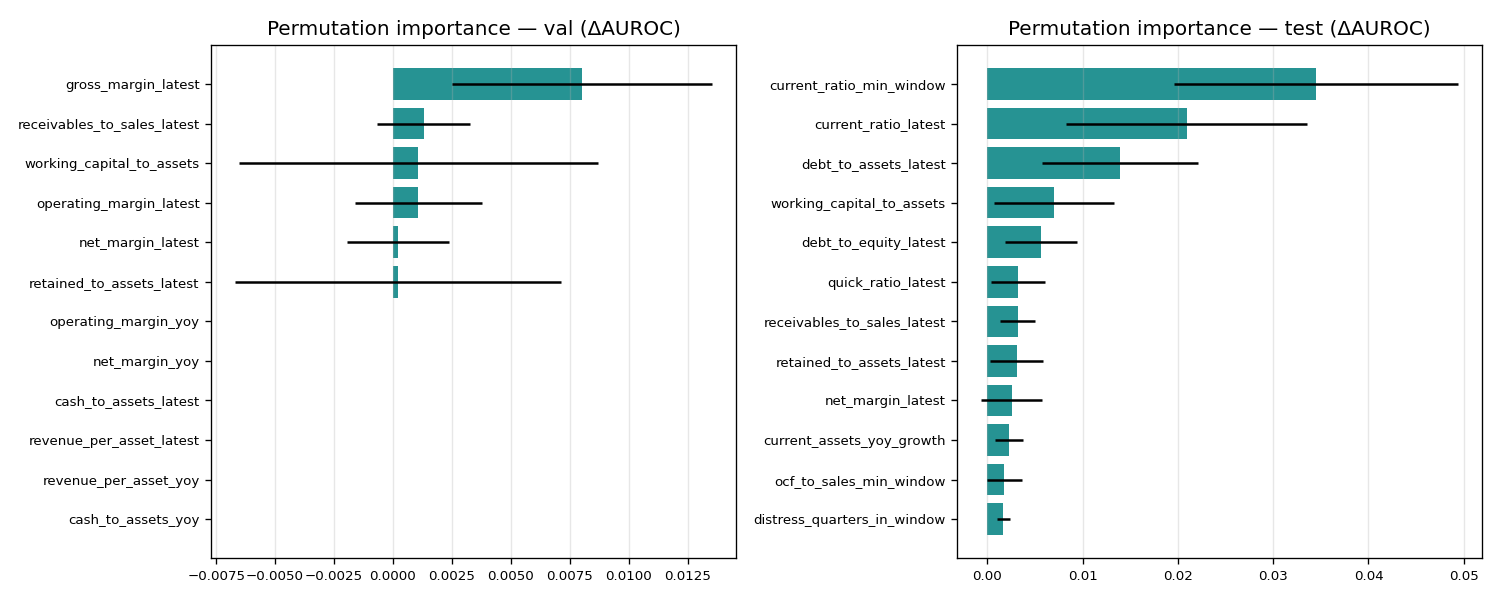
\includegraphics[width=0.8\textwidth]{figures/02_feature_importance.png}
\caption{Độ quan trọng đặc trưng (permutation)}
\end{figure}

\begin{table}[H]
\centering
\caption{Ablation theo nhóm đặc trưng (test)}
\begin{center}
\footnotesize
\begin{tabular}{|l|c|c|c|c|}
\hline
\textbf{Biến thể} & \textbf{Số đặc trưng} & \textbf{AUROC test} & \textbf{AP test} & \textbf{F1 test} \\ \hline
Tất cả đặc trưng & 47 & 0,983 & 0,991 & 0,949 \\ \hline
Bỏ nhóm ratios\_latest & 33 & 0,966 & 0,982 & 0,949 \\ \hline
Bỏ nhóm ratios\_yoy & 33 & 0,974 & 0,985 & 0,949 \\ \hline
Bỏ nhóm growth & 37 & 0,985 & 0,993 & 0,949 \\ \hline
Bỏ nhóm path & 41 & 0,977 & 0,987 & 0,949 \\ \hline
Chỉ mẫu có ≥ 5 quý lịch sử & 47 & 0,987 & 0,993 & 0,949 \\ \hline
\end{tabular}
\end{center}
\end{table}

Ablation cho thấy F1 test gần như không đổi (0,949) ở mọi biến thể, còn AUROC dao động trong khoảng ±0,02 — tức kết luận không nhạy với việc bỏ nguyên một nhóm đặc trưng. Bỏ nhóm \texttt{ratios\_latest} làm AUROC giảm nhiều nhất (0,983 → 0,966), cho thấy giá trị tỷ số tại quý gần nhất là phần thông tin cốt lõi. Một cảnh báo kỹ thuật đi kèm: đa cộng tuyến cao — 33/47 đặc trưng có VIF > 10 (nặng nhất \texttt{debt\_to\_equity} và các cột \texttt{cash\_*}). Với mô hình tuyến tính, VIF cao làm hệ số bất ổn và khó diễn giải; với mô hình cây thì ít ảnh hưởng đến dự báo nhưng vẫn làm độ quan trọng bị chia đều giữa các cột tương quan.

\begin{figure}[H]
\centering
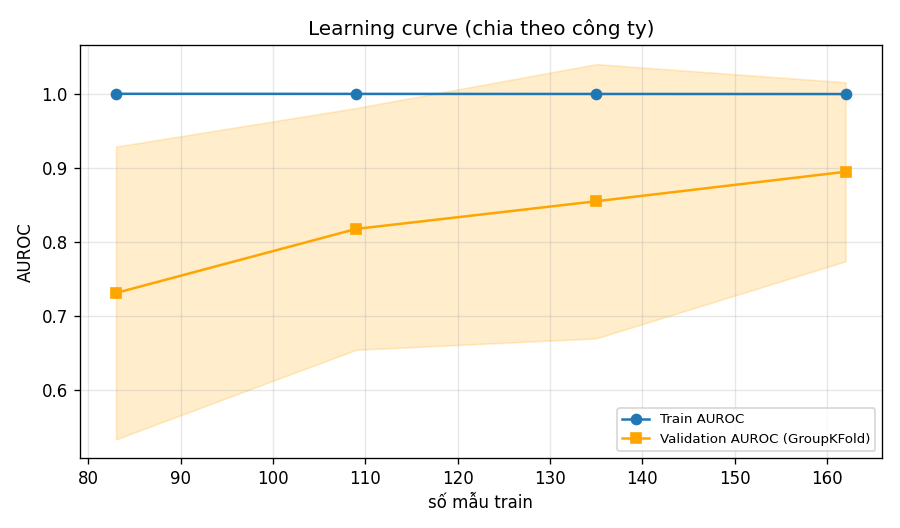
\includegraphics[width=0.8\textwidth]{figures/06_learning_curve.png}
\caption{Learning curve khi chia theo công ty}
\end{figure}

\clearpage

\subsection{Kiểm định ý nghĩa thống kê và độ nhạy theo định nghĩa nhãn}

Để tránh kết luận 'mô hình tốt hơn' chỉ dựa vào chênh lệch điểm số, nhóm kiểm định trên cùng 64 mẫu test: DeLong (1988) cho ΔAUROC và paired bootstrap (2.000 vòng) cho ΔAP.

\begin{table}[H]
\centering
\caption{Kiểm định mô hình chốt so với các hệ thống khác}
\begin{center}
\footnotesize
\begin{tabular}{|l|c|c|c|c|c|}
\hline
\textbf{So sánh (A − B)} & \textbf{ΔAUROC} & \textbf{p (DeLong)} & \textbf{ΔAP} & \textbf{CI95 ΔAP} & \textbf{p (bootstrap)} \\ \hline
RF − ticker\_prior & −0,0030 & 0,755 & +0,0061 & [−0,005; +0,022] & 0,344 \\ \hline
RF − single\_feature & +0,0941 & 0,0076 & +0,0528 & [+0,018; +0,097] & 0,001 \\ \hline
RF − dummy\_most\_frequent & +0,4828 & <0,001 & +0,3970 & [+0,379; +0,406] & <0,001 \\ \hline
\end{tabular}
\end{center}
\end{table}

Kết quả then chốt: mô hình chốt \textbf{không} khác baseline ticker-prior về ý nghĩa thống kê (p = 0,755 cho AUROC; p = 0,344 cho AP, khoảng tin cậy chứa 0). Cần đọc đúng: 'không khác biệt' nghĩa là dữ liệu chưa đủ để khẳng định mô hình hơn, không phải bằng chứng mô hình kém. Với n = 64, khoảng tin cậy vốn rộng. Đây chính là lý do nhóm đặt baseline làm mốc trung thực thay vì chỉ so giữa các mô hình với nhau.

Phép thử thứ hai kiểm tra kết luận có phụ thuộc vào cách gán nhãn không. Nhóm dựng lại toàn bộ split bằng ba định nghĩa nhãn công khai, tái lập được (stress\_signals, Altman Z'', forward 4 quý) và chạy lại đúng một mô hình:

\begin{table}[H]
\centering
\caption{Kiểm chứng độ nhạy theo định nghĩa nhãn}
\begin{center}
\footnotesize
\begin{tabular}{|l|c|c|c|c|c|}
\hline
\textbf{Định nghĩa nhãn} & \textbf{Dương (test)} & \textbf{Khớp nhãn gốc} & \textbf{AUROC mô hình} & \textbf{AUROC ticker-prior} & \textbf{Cross-co. AP} \\ \hline
original (nhãn gốc) & 59,4\% & 100\% & 0,983 & 0,986 & 0,958 \\ \hline
stress\_signals & 42,2\% & 74,4\% & 0,909 & 0,960 & 0,610 \\ \hline
altman\_z & 31,2\% & 63,9\% & 0,999 & 0,991 & 0,460 \\ \hline
forward\_4q & 48,4\% & 66,7\% & 0,836 & 0,911 & 0,582 \\ \hline
\end{tabular}
\end{center}
\end{table}

Luận điểm 'mô hình không vượt baseline nhớ mặt công ty' xuất hiện ở \textbf{3/3} định nghĩa nhãn tái lập được — đây là bằng chứng mạnh nhất của đồ án: kết luận không phụ thuộc vào cách gán nhãn. Đồng thời, cross-company AP sụt rất mạnh ở các định nghĩa khác (0,46–0,61), xác nhận lại rằng phần lớn hiệu năng in-domain đến từ thực thể chứ không từ động lực suy giảm của từng quý.

\subsection{Thực nghiệm phản biện (LiteSVM, XGBoost)}

Để trả lời câu hỏi 'có phải do chọn họ mô hình nên chưa hơn baseline?', nhóm chạy thêm hai đối chứng ngoài pipeline chính: một SVM tuyến tính nhẹ (LiteSVM, cài bằng numpy) và XGBoost:

\begin{table}[H]
\centering
\caption{Mô hình chốt so với LiteSVM và XGBoost (test)}
\begin{center}
\small
\begin{tabular}{|l|c|c|c|}
\hline
\textbf{Mô hình} & \textbf{Test AUROC} & \textbf{Test AP} & \textbf{TN/FP/FN/TP} \\ \hline
LiteSVM (SGD hinge + class\_weight) & 0,965 & 0,976 & 26/0/19/19 \\ \hline
XGBoost (scale\_pos\_weight + early stopping) & 0,982 & 0,990 & 26/0/4/34 \\ \hline
Random Forest (đồ án) & 0,983 & 0,991 & 25/1/2/36 \\ \hline
\end{tabular}
\end{center}
\end{table}

XGBoost đạt AUROC/AP tương đương Random Forest trong khi không FP nào (bỏ sót 4) — nghĩa là việc thay boosting bằng bagging không tạo khác biệt lớn trên bộ dữ liệu này. Kiểm định cặp giữa hai mô hình cho thấy chênh lệch không có ý nghĩa thống kê. Kết luận: nút thắt không nằm ở thuật toán mà ở dữ liệu (8 thực thể) và định nghĩa nhãn. Nhóm cũng chạy thí nghiệm xử lý mất cân bằng trên dữ liệu thật (SMOTE, SMOTE+ENN, RandomUnderSampler, class\_weight) đặt trong \texttt{imblearn.pipeline.Pipeline} để không chạm test; kỹ thuật tốt nhất (\texttt{smote\_enn}, AP 0,9683 so với 0,9588 của đối chứng) nhưng ΔAP = +0,0095 với p = 0,21 — chưa đủ căn cứ. Một chi tiết đáng lưu ý: vì lớp 1 chiếm đa số (62\%), SMOTE ở đây sinh thêm mẫu lớp 0, tức can thiệp ngược với thực hành phổ biến — thêm một lý do để mất cân bằng không phải nút thắt của bài toán này.

\clearpage

\chapter{THẢO LUẬN VÀ ĐÁNH GIÁ}

\section{Ý nghĩa thực tiễn}

Giá trị thực dụng rõ nhất của đồ án không nằm ở con số AUROC 0,983, mà ở hai thứ khác. Một là khả năng tự động hoá bóc tách: thay vì đọc 8×44 báo cáo, pipeline lấy thẳng \texttt{companyfacts}, chuẩn hoá kỳ kế toán, tính 47 đặc trưng và gán nhãn, tất cả tái lập được từ một lệnh. Với đơn vị muốn sàng lọc rủi ro theo quý trên hàng trăm mã, đây là phần tiết kiệm thời gian thật.

Hai là phát hiện trung thực về rò rỉ cấp thực thể. Với dữ liệu chỉ có 8 công ty, một mô hình học có thể đạt AUROC ≈ 0,98 trong kiểm định thông thường mà phần lớn năng lực chỉ là 'nhớ mặt công ty'. Bất kỳ ai triển khai dự báo suy giảm trên bộ dữ liệu ít thực thể đều cần biết điều này; đồ án định lượng nó (in-domain 0,983 so với cross-company 0,933) và đề xuất giao thức đo đúng thay vì chỉ đưa ra một con số đẹp.

\section{Phân tích lỗi (error analysis)}

Trên test, mô hình chốt sai 3/64 mẫu. Nhóm truy vết từng ca tới chỉ tiêu cụ thể:

\begin{table}[H]
\centering
\caption{Ba mẫu dự đoán sai trên test}
\begin{center}
\footnotesize
\begin{tabular}{|l|c|c|c|c|c|c|c|c|}
\hline
\textbf{Mẫu} & \textbf{Công ty} & \textbf{Thực tế} & \textbf{Dự đoán} & \textbf{P(distress)} & \textbf{current\_ratio} & \textbf{WC/assets} & \textbf{net\_margin} & \textbf{debt/assets} \\ \hline
HD-2024Q2 & HD & 1 & 0 (FN) & 0,783 & 1,34 & 0,10 & 0,099 & 0,98 \\ \hline
DG-2025Q2 & DG & 0 & 1 (FP) & 0,798 & 1,23 & 0,05 & 0,038 & 0,75 \\ \hline
FIVE-2024Q3 & FIVE & 1 & 0 (FN) & 0,174 & 1,63 & 0,11 & 0,040 & 0,60 \\ \hline
\end{tabular}
\end{center}
\end{table}

Ba ca này lộ ra đúng bản chất vấn đề. \texttt{HD-2024Q2} là bỏ sót sát ngưỡng: HD có 100\% quý mang nhãn 1, nhưng quý này các tỷ số lại khá hơn (net\_margin 0,099; debt/assets 0,98) nên xác suất 0,783 nằm ngay dưới ngưỡng 0,788 — mô hình gần như dựa vào danh tính công ty chứ không vào tín hiệu của quý. \texttt{FIVE-2024Q3} là bỏ sót nặng (0,174): đây là lỗi đáng lo nhất, vì mô hình không hề thấy dấu hiệu nào. \texttt{DG-2025Q2} là báo động giả (0,798) ở một công ty có nhãn lẫn lộn. Điểm chung: cả ba mẫu đều thuộc các công ty có tỉ lệ nhãn trung gian, nơi ranh giới quyết định mờ.

\section{Rào cản kỹ thuật khi triển khai thực tế}

\begin{enumerate}
\item \textbf{Độ trễ dữ liệu theo quý.} Đầu vào là báo cáo quý đã công bố. 10-Q thường nộp sau khi quý kết thúc khoảng 40 ngày, 10-K có kiểm toán; mọi đặc trưng trong đồ án dùng mốc \texttt{available\_on} = ngày \texttt{filed}. Điều đó có nghĩa dự báo chỉ có thể đưa ra SAU khi báo cáo được nộp — mô hình không thể cảnh báo sớm hơn chính dữ liệu. Tệ hơn, các tỷ số kế toán là chỉ báo trễ: khi chúng xấu đi thì vấn đề thường đã xảy ra rồi.
\item \textbf{Rò rỉ cấp thực thể.} Đây là rủi ro lớn nhất về phương pháp. Nếu chia tập ngẫu nhiên theo mẫu, cùng một công ty xuất hiện ở cả train lẫn test và mô hình chỉ cần nhớ mặt công ty là đủ đạt điểm cao giả tạo. Đồ án tránh bằng chia theo thời gian + GroupKFold/LOCO và luôn so với baseline ticker-prior.
\item \textbf{Chi phí sai không đối xứng.} Trong ứng dụng đầu tư/cho vay, một FN (bỏ sót doanh nghiệp sắp suy giảm) đắt hơn một FP. Đồ án xử lý bằng ngưỡng tối ưu chi phí, nhưng giả định \texttt{COST\_FN = 5} là con số minh hoạ, không phải con số đo được từ thị trường.
\item \textbf{Nhãn mục tiêu không tái tạo được.} Không quy tắc kế toán đơn giản nào khớp nhãn gốc quá 74,7\%. Điều này giới hạn khả năng kiểm chứng độc lập và buộc đồ án phải kiểm chứng độ nhạy bằng các định nghĩa nhãn thay thế.
\item \textbf{Nguy cơ overfitting.} Random Forest đạt AUROC train 1,000 nhưng validation 0,965 (gap 0,034); learning curve chia theo công ty cho gap khoảng 0,105 AUROC. Với 212 mẫu train và 47 đặc trưng, đây là mức overfit cần theo dõi, và là lý do nhóm không dùng cấu hình tinh chỉnh phức tạp.
\end{enumerate}

\section{Hạn chế của bộ dữ liệu và phạm vi kết luận}

Nhóm nêu rõ các giới hạn thay vì che đi. Cỡ mẫu nhỏ và chỉ 8 thực thể: mọi kết luận phải đi kèm khoảng tin cậy và không suy rộng ra toàn ngành. Chuỗi thời gian bị chồng lấn giữa các mẫu liên tiếp (cùng một quý xuất hiện trong nhiều cửa sổ lịch sử) nên số quan sát độc lập thực tế nhỏ hơn 324. Nhãn gốc không tái tạo được. Đơn vị tiền chỉ là quy đổi minh hoạ. Và quan trọng nhất: bộ dữ liệu không chứa sự kiện phá sản thật, nên kết quả không thể diễn giải thành năng lực dự báo phá sản.

\clearpage

\chapter{KẾT LUẬN VÀ HƯỚNG PHÁT TRIỂN}

\section{Kết luận}

Đồ án đã làm được những việc cụ thể và chưa chứng minh được một điều quan trọng. Về phần đã làm:

\begin{enumerate}
\item Pipeline dữ liệu SEC XBRL tái lập được: 8 công ty, 332 quý, 16 chỉ tiêu, kiểm chứng provenance bằng SHA-256 (0 hash lệch, 0 fact thiếu, 0 ô bịa số).
\item Bộ 47 đặc trưng tài chính gồm tỷ số thanh khoản/đòn bẩy/sinh lời/hiệu quả, tăng trưởng YoY và đặc trưng đường đi theo cửa sổ quý.
\item Bốn họ mô hình scikit-learn đặt trong một Pipeline chống rò rỉ, cộng các baseline đối chứng (dummy, ticker-prior, single-feature, Altman Z'').
\item Kết quả test: Random Forest được chốt đạt AUROC 0,983, AP 0,991, F1 0,960 tại ngưỡng 0,788.
\item Ba lớp kiểm chứng: cross-company/LOCO, kiểm định ý nghĩa (DeLong + bootstrap), và kiểm chứng độ nhạy theo 3 định nghĩa nhãn tái lập được.
\end{enumerate}

Về phần chưa chứng minh được — và đây là kết luận trung thực quan trọng nhất: trên bộ test 64 mẫu, mô hình \textbf{không} vượt baseline ticker-prior về ý nghĩa thống kê, và năng lực tổng quát hoá sang công ty chưa từng thấy còn thấp (cross-company AUROC 0,933; LOCO 0,628). Nút thắt của bài toán không nằm ở thuật toán: đổi Random Forest sang XGBoost hay LiteSVM, hay thêm SMOTE, đều không tạo khác biệt có ý nghĩa. Nút thắt nằm ở dữ liệu (chỉ 8 thực thể) và ở định nghĩa nhãn.

\section{Hướng phát triển}

\begin{enumerate}
\item \textbf{Khai thác văn bản 10-K/10-Q (NLP).} Phần thuyết minh MD\&A và ghi chú thường chứa cảnh báo định tính (going concern, kiện tụng, mất khách hàng lớn) mà các tỷ số kế toán bỏ sót. Đây là hướng bổ sung thông tin mạnh nhất, vì nó thêm loại tín hiệu khác về bản chất chứ không thêm biến thể của cùng một loại.
\item \textbf{Thêm dữ liệu thị trường theo thời gian thực.} Giá cổ phiếu, spread tín dụng (CDS), lợi suất trái phiếu doanh nghiệp và biến động ngụ ý cập nhật liên tục — thay cho dữ liệu kế toán trễ theo quý. Kết hợp hai loại tín hiệu có thể giảm độ trễ cảnh báo.
\item \textbf{Mở rộng universe và thêm ngành.} Tăng số thực thể (nhiều công ty bán lẻ hơn, hoặc nhiều ngành) để cross-company học được quy luật chung thay vì nhớ mặt công ty.
\item \textbf{Mô hình hoá theo thời gian (survival/sequence).} Thay phân loại từng quý bằng mô hình survival hoặc chuỗi (LSTM, Temporal Fusion) khai thác tính chồng lấn của chuỗi thời gian và dự báo thời điểm xảy ra suy giảm thay vì chỉ xác suất một quý.
\item \textbf{Bổ sung sự kiện phá sản thật.} Mở rộng tập sang các công ty đã nộp 8-K item 1.03 để có nhãn kiểm chứng được, từ đó chuyển bài toán sang dự báo phá sản thật sự.
\end{enumerate}

\clearpage


\chapter*{TÀI LIỆU THAM KHẢO}
\addcontentsline{toc}{chapter}{Tài liệu tham khảo}
\begin{thebibliography}{99}
\bibitem{beaver1966} W. H. Beaver, ``Financial ratios as predictors of failure,'' \emph{Journal of
Accounting Research}, vol. 4, pp. 71--111, 1966.
\bibitem{altman1968} E. I. Altman, ``Financial ratios, discriminant analysis and the prediction of
corporate bankruptcy,'' \emph{The Journal of Finance}, vol. 23, no. 4, pp. 589--609, 1968.
\bibitem{altman2000} E. I. Altman, ``Predicting financial distress of companies: Revisiting the
Z-score and ZETA models,'' Working paper, 2000.
\bibitem{barboza2017} F. Barboza, H. Kimura, and E. Altman, ``Machine learning models and bankruptcy
prediction,'' \emph{Expert Systems with Applications}, vol. 83, pp. 405--417, 2017.
\bibitem{pedregosa2011} F. Pedregosa et al., ``Scikit-learn: Machine learning in Python,''
\emph{Journal of Machine Learning Research}, vol. 12, pp. 2825--2830, 2011.
\bibitem{breiman2001} L. Breiman, ``Random forests,'' \emph{Machine Learning}, vol. 45, no. 1,
pp. 5--32, 2001.
\bibitem{friedman2001} J. H. Friedman, ``Greedy function approximation: A gradient boosting
machine,'' \emph{Annals of Statistics}, vol. 29, no. 5, pp. 1189--1232, 2001.
\bibitem{chen2016} T. Chen and C. Guestrin, ``XGBoost: A scalable tree boosting system,'' in
\emph{Proc. ACM SIGKDD}, 2016, pp. 785--794.
\bibitem{fawcett2006} T. Fawcett, ``An introduction to ROC analysis,'' \emph{Pattern Recognition
Letters}, vol. 27, no. 8, pp. 861--874, 2006.
\bibitem{davis2006} J. Davis and M. Goadrich, ``The relationship between Precision-Recall and ROC
curves,'' in \emph{Proc. ICML}, 2006, pp. 233--240.
\bibitem{delong1988} E. R. DeLong, D. M. DeLong, and D. L. Clarke-Pearson, ``Comparing the areas
under two or more correlated receiver operating characteristic curves,'' \emph{Biometrics}, vol. 44,
no. 3, pp. 837--845, 1988.
\bibitem{chawla2002} N. V. Chawla et al., ``SMOTE: Synthetic Minority Over-sampling Technique,''
\emph{Journal of Artificial Intelligence Research}, vol. 16, pp. 321--357, 2002.
\bibitem{lemaitre2017} G. Lema\^{i}tre, F. Nogueira, and C. K. Aridas, ``Imbalanced-learn: A Python
toolbox to tackle the curse of imbalanced datasets,'' \emph{Journal of Machine Learning Research},
vol. 18, pp. 1--5, 2017.
\bibitem{lundberg2017} S. M. Lundberg and S.-I. Lee, ``A unified approach to interpreting model
predictions,'' in \emph{Proc. NeurIPS}, 2017, pp. 4765--4774.
\bibitem{fisher2019} A. Fisher, C. Rudin, and F. Dominici, ``All models are wrong, but many are
useful: Learning a variable's importance by studying an entire class of prediction models,''
\emph{Journal of Machine Learning Research}, vol. 20, pp. 1--81, 2019.
\bibitem{secxbrl2026} U.S. Securities and Exchange Commission, ``Structured data / XBRL,''
\url{https://www.sec.gov/structureddata} (truy cập 2026).
\bibitem{secfacts2026} U.S. Securities and Exchange Commission, ``SEC EDGAR XBRL company facts
API,'' \url{https://data.sec.gov/api/xbrl/companyfacts/} (truy cập 2026).
\end{thebibliography}


\end{document}